\documentclass[prd,twocolumn,tightenlines,preprintnumbers,showpacs,superscriptaddress,notitlepage,nofootinbib,eqsecnum,floatfix,longbibliography]{revtex4}
\usepackage[utf8]{inputenc}
\usepackage[T1]{fontenc}
\usepackage{amsmath,amssymb}
\usepackage{bm,bbm}
\usepackage{graphicx}
\usepackage{color}
\usepackage{dsfont}

\usepackage{hyperref}
\hypersetup{
    colorlinks=true,       % false: boxed links; true: colored links
    linkcolor=blue,          % color of internal links
    citecolor=blue,        % color of links to bibliography
    filecolor=blue,      % color of file links
    urlcolor=blue           % color of external links
}

\begin{document}
\title{Solutions to Integer Programming from Quantum Annealing}

\author{Chia~Cheng~Chang}
\affiliation{RIKEN Interdisciplinary Theoretical and Mathematical Sciences (iTHEMS), Wako, Saitama 351-0198, Japan}
\affiliation{Department of Physics, University of California, Berkeley, California 94720, USA}
\affiliation{Nuclear Science Division, Lawrence Berkeley National Laboratory, Berkeley, California 94720, USA}
\author{Chih-Chieh~Chen}
\affiliation{R\&D Group, Grid Inc., Tokyo 107-0061, Japan}
\author{Christopher K\"orber}
\affiliation{Department of Physics, University of California, Berkeley, California 94720, USA}
\affiliation{Nuclear Science Division, Lawrence Berkeley National Laboratory, Berkeley, California 94720, USA}
\author{Travis~Humble}
\affiliation{Quantum Computing Institute, Oak Ridge National Laboratory, Oak Ridge, Tennessee 37831, USA}
\author{Jim~Ostrowski}
\affiliation{University of Tennessee}

\begin{abstract}
Abstract here...
\end{abstract}

\preprint{LLNL-JRNL-809712, RIKEN-iTHEMS-Report-20}

\maketitle
%%%%%%%%%%%%%%%%%%%%%%%%%%%%%%%%%
%%%%%%%%%%%%%%%%%%%%%%%%%%%%%%%%%
%%%%%%%%%%%%%%%%%%%%%%%%%%%%%%%%%
\tableofcontents

\flushbottom
\maketitle

\section{INTRODUCTION}
\label{sec:introduction}

Integer linear programming (ILP) is an integer optimization problem subject to inequality constraints and is a commonly tackled problem applicable to situations such as x~\cite{}, y~\cite{}, and z~\cite{}. In general however, ILP is classically NP-complete, and as a result, heuristic methods are employed~\cite{}. The NP-hardness of ILP can be understood by realizing that while the solution to an $n$-dimensional linear problem can be obtained in polynomial time, the optimal integer solution in general must be found in the $2^n$ integer solutions which surround the real number solution. Due to the importance and difficulty, in this work we present a method to obtain the optimal solution to ILP by employing methods of quantum annealing.

Quantum annealing solves a general quadratic binary optimization problem (QUBO) by slowly varying a time-dependent Hamiltonian~\cite{}. Through the adiabatic theorem of quantum mechanics, the annealer is prepared initially in a trivial ground state while the solution to ILP is encoded in the target Hamiltonian. Due to the explosion in research efforts towards hardware implementations of quantum annealers and future improvements to the annealing schedule~\cite{}, mapping ILP to QUBO provides a path forward towards obtaining optimal solutions to the class of integer optimization problems~\cite{2018Glover}.

Formally, ILP is defined as the optimization of a linear function
\begin{align}
f(x) = &\min\limits_{x}(c_i x_i),\\
\textrm{subject to} \quad & A_{aj}x_i +b_a \leq 0 \\
& x_i \geq 0,\\
& x_i \in \mathbb{Z}
\end{align}
where $i=1, \cdots,  N$ is the number of dependent variables and $a=1, \cdots, M$ the number of constraint equations. The inequality constraints can be rewritten as an equality by introducing slack variables $s$ such that the ILP becomes
\begin{align}
f(x) = &\min(c_i x_i),\\
\textrm{subject to} \quad & A_{a i}x_i + s_a + b_a = 0,\\
& s_a \geq 0,\\
& s_a \in \mathbb{Z},\\
& x_i \geq 0,\\
& x_i \in \mathbb{Z}.
\end{align}

Since quantum annealing solves the QUBO problem, we extend the proposed algorithm to solve integer quadratic optimization problems such that
\begin{align}
f(x) = \min\limits_{x}(x_i d_{ij} x_j + c_i x_i)
\end{align}
without the introduction of auxiliary qubits.

{\color{red} Paragraph on how this is solved classically. Include strengths and drawbacks of classical solution.}

\section{RESULTS}
\label{sec:results}
We map integer variables $z_i$ to qubits under the following transformation~\cite{Chang:2018uoc}
\begin{align}
z_i = & \sum_{r=0}^{R_i-1} 2^r \psi_{ri}
\label{eq:int_to_bin}
\end{align}
where $\psi_{ri} \in \{0, 1\}$ while the number of qubits used to represent the $i$-th integer variable is allowed to vary with $R_i$. The transformation can in general be express as a rectangular matrix. For example, a vector of two integer variables $z_0$ and $z_1$ represented by one and two qubits respectively is given as
\begin{align}
\begin{pmatrix}
z_0\\
z_1
\end{pmatrix}
= &
\begin{pmatrix}
2^0 & 0 & 0\\
0 & 2^0 & 2^1
\end{pmatrix}
\begin{pmatrix}
\psi_{00}\\
\psi_{01}\\
\psi_{11}
\end{pmatrix}
\equiv T^z \begin{pmatrix}
\psi_{00}\\
\psi_{01}\\
\psi_{11}
\end{pmatrix}
\end{align}
The transformation can be reduced to a tensor product if $R_i$ is a constant for all $i$ such that
\begin{align}
\mathcal{R} = & \begin{pmatrix} 2^0 & \dots & 2^{R-1}\end{pmatrix},\\
\mathcal{Z} = & \begin{pmatrix} z_0 & \dots & z_{N-1}\end{pmatrix},\\
|\mathds{1}| = & |\mathcal{Z}|,\\
T^z = & \mathds{1}\otimes \mathcal{R}.
\end{align}

While the coefficients of the inequality constraints are not required to be integer valued, the inequalities can be trivially rescaled such that $s_i \in \mathbb{Z}$ given fixed precision coefficients $A_{ij}$ and $b_i$. As a result, we can restrict both $x_i$ and $s_i$ to sample over only positive integer values as allowed by Eq.~(\ref{eq:int_to_bin}).

\subsection{Integer Programming Mapping to QUBO}
\label{sec:results:ilp}
The integer quadratic optimization problem can be mapped to a minimization of the quadratic objective function
\begin{align}
\chi^2 = & \left[\Psi^x_{\mu} T^x_{\mu i}d_{ij} T^x_{j \nu}\Psi^x_\nu + c_i T^x_{i\mu} \Psi^x_\mu \right. \nonumber\\
&\left.+ p (A_{a b} T^x_{b \mu} \Psi^x_{\mu} + T^s_{a \alpha} \Psi^s_\alpha + b_a)^2 \right],\\
\Psi = & \begin{pmatrix}
\Psi^x\\
\Psi^s
\end{pmatrix},
\end{align}
where $p$ is the strength of the penalty factor which must be set large enough such that the constraints are satisfied under minimization. The objective function can be represented as a QUBO Hamiltonian
\begin{align}
E = &
\begin{pmatrix}
\Psi^x & \Psi^s
\end{pmatrix}
\begin{pmatrix}
Q_{xx} & Q_{xs}\\
Q_{sx} & Q_{ss} 
\end{pmatrix}
\begin{pmatrix}
\Psi^x\\ \Psi^s
\end{pmatrix} + pb^2,\\
\equiv & \Psi^T Q \Psi + C,
\label{eq:matrix_form}
\end{align}
where
\begin{align}
Q_{xx} = & {T^{x}}^T \left[ d + p A^T A + p \mathrm{Diag}_{x} \left(A^T b + b^T A\right) \right] T^x \nonumber \\
&+ \mathrm{Diag}_{\psi^x}(c) T^x,\\
Q_{xs} = & Q_{sx}^T = p {T^{x}}^T A^T T^s,\\
Q_{ss} = & p\left[ {T^{s}}^T T^s + \mathrm{Diag}_{\psi^s}\left( {T^{s}}^T b + b^T T^s\right) \right].
\end{align}
The function $\mathrm{Diag}_{z}(v)$ embeds a vector $v$ into a diagonal matrix in subspace $z$, and absorbs the linear contributions of the QUBO into the diagonal elements of the quadratic representation.

\subsection{Application to the Dominating Set Problem}
\label{sec:results:mds}

Given a graph $G(E,V)$, defined by the set of $V$ vertices and $E$ edges, and a subset of vertices $D \subseteq V$. If the set of all vertices not in $D$ is adjacent to at least one vertex in $D$, then $D$ is a dominating set. This is equivalent to requiring the set of nearest-neighbor vertices of $D$ (exclusive) and $D$ cover all vertices $N(D) \cup D = V$ (an example is given by Fig.~\ref{fig:dominating_sets}a). The set $D$ is a minimal dominating set if there is no proper subset of $D$ that is a dominating set, {\it{i.e.}}, the removal of any vertex in $D$ results in $N(D) \cup D  \neq V$. An example is given by Fig.~\ref{fig:dominating_sets}b. The domination number of $D$ is given by the cardinality of $|D| \equiv \overline{\overline{D}}$. The minimum dominating set (MDS) is defined by $D$ with the smallest domination number. Fig.~\ref{fig:dominating_sets}c shows an example of the minimum dominating set of $G(V, E)$ and is different from the minimal dominating set. We emphasize that while the maximum independent set is always a minimal dominating set as exemplified by Fig.~\ref{fig:dominating_sets}b, the minimum dominating set in general can have a smaller domination number. As a result, the solution to the dominating set problem can not be obtained by solving for the maximum independent set, a problem that is well studied for quantum annealers~\cite{}.

\begin{figure*}
	\centering
	\begin{tabular}{p{0.3\textwidth}p{0.3\textwidth}p{0.3\textwidth}}
	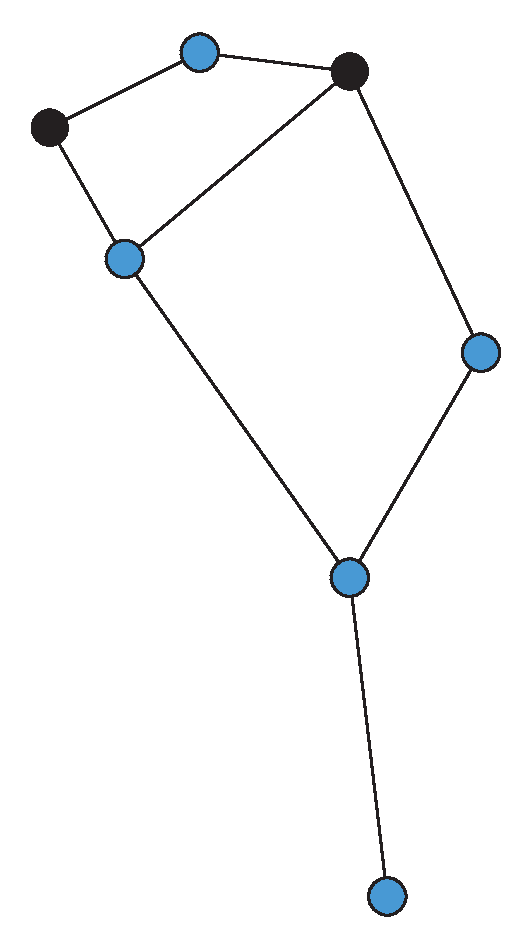
\includegraphics[width=0.20\textwidth]{./figures/subaru_ds.pdf}
&
	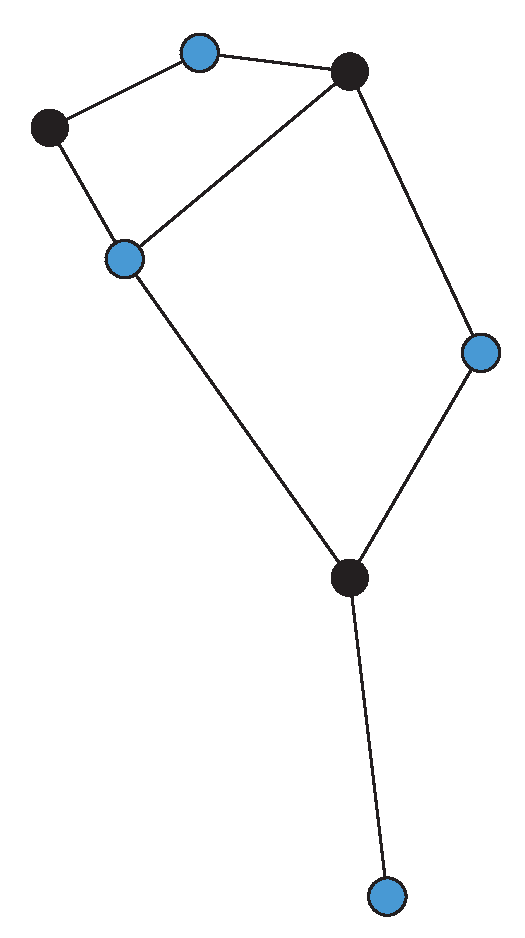
\includegraphics[width=0.20\textwidth]{./figures/subaru_mds4.pdf}
&
	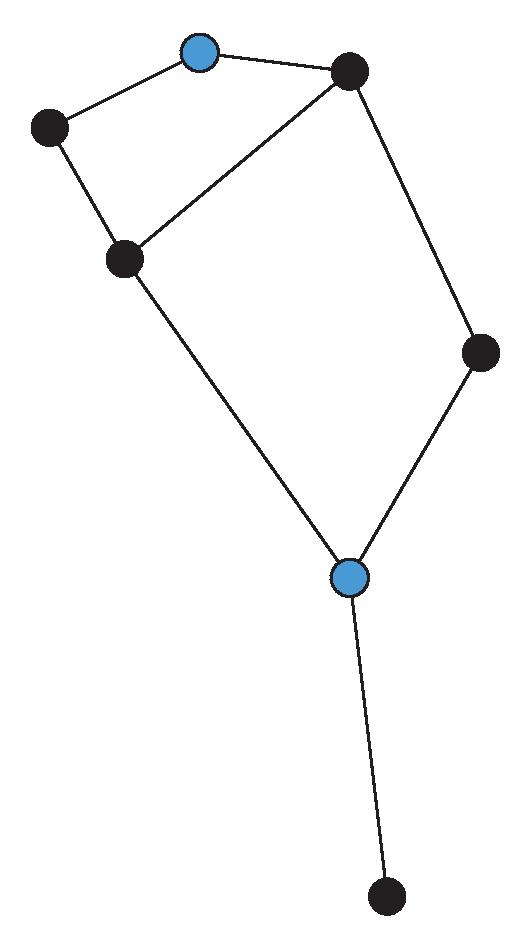
\includegraphics[width=0.20\textwidth]{./figures/subaru_mds2.pdf}\\
	\centering\bf{a} & \centering\bf{b} & \centering\bf{c}
	\end{tabular}
	\caption{Example of different dominating sets for the Pleiades constellation $G(V, E)$. Vertices in the dominating set $D$ are highlighted in blue. {\bf{a)}} A dominating set of $G$ with domination number $\overline{\overline{D}} = 5$. {\bf{b)}} A minimal dominating set of $G$ with domination number of $\overline{\overline{D}} = 4$. We note that $D$ is also the maximum independent set of $G$. {\bf{c)}} The minimum dominating set of $G$ with domination number of $\overline{\overline{D}} = 2$.}
	\label{fig:dominating_sets}
\end{figure*}

For general graphs, existing "classical" algorithms either find minimal solutions in exponential time $\sim O( 1.5^n)$ \cite{Fomin2009, vanRooij2009} or approximate solutions in polynomial time. For example, greedy algorithms locally optimize decisions about which nodes to add to the dominating set.
Thus one is guaranteed to find a dominating set but not necessarily a MDS.
We demonstrate an example greedy algorithm in figure Fig.~\ref{fig:mds-greedy}.
\begin{figure*}
	\centering
	\begin{tabular}{p{0.22\textwidth}p{0.22\textwidth}p{0.22\textwidth}p{0.22\textwidth}}
	\includegraphics[width=0.20\textwidth]{./figures/greedy-1.pdf}
&
	\includegraphics[width=0.20\textwidth]{./figures/greedy-2.pdf}
&
	\includegraphics[width=0.20\textwidth]{./figures/greedy-3.pdf}
&
	\includegraphics[width=0.20\textwidth]{./figures/greedy-4.pdf}\\
	\centering\bf{a} & \centering\bf{b} & \centering\bf{c} & \centering\bf{d}
	\end{tabular}
	\caption{
		Example of greedy MDS algorithm:
		The algorithm iteratively adds vertices to the dominating set (black nodes) such that newly added nodes are maximally unconnected (white nodes).
		Connected nodes are neighbors of the DS (turquoise) or already in the DS.
		In (a), one finds three unconnected nodes [(2), (4), (7)] which are adjacent to three unconnected nodes each.
		In the first step $a\to b$, randomly the node (4) is picked.
		In (b), one has two unconnected choices [(1), (2)] with each adjacent to another unconnected node.
		After randomly selecting (2) when going from $b \to c$, only one unconnected node is remaining (6).
		The found solution is a (minimal) dominating set but not a MDS.
		To find the MDS using this greedy algorithm, the first node choice must be either (2) or (5).
	}
	\label{fig:mds-greedy}
\end{figure*}

\subsubsection{Minimum Dominating Set}
The solution to the minimum independent set can be expressed as an integer optimization problem given by,
\begin{align}
f(x) = &\min(\sum_{\nu \in V} \psi^x_{\nu}),\\
\textrm{subject to} \quad & \psi^x_{\nu} + \sum_{\mu \in \mathit{N}(\nu)} \psi^x_{\mu} \geq 1,\\
& \psi^x_{\nu} \in \{0, 1\}
\end{align}
where the dimension of the dependent variable $x$ is the number of vertices $\overline{\overline{V}}$.
The problem minimizes the number of vertices in $D$ with a binary variable $\psi^x$ encoded by a single qubit, subject to the constraint that at least one vertex in $\mathit{N}(\nu)$ is in $D$. For each vertex in $V$ we introduce slack variables $s_{\nu} = T^s_{\nu \alpha} \psi^s_{\alpha}$ to encode the inequality constraint such that
\begin{align}
f(x) = &\min(\sum_{\nu\in V} \psi^x_{\nu}),\\
\textrm{subject to} \quad & \psi^x_{\nu} + J_{\nu \mu} \psi^x_{\mu}- T^s_{\nu \alpha} \psi^s_{\alpha}  - 1 = 0,\\
& \psi_{\nu} \in \{0, 1\},\\
& 0 \leq s_{\nu} \leq |\mathrm{N}(\nu)|\\
& s_{\nu} \in \mathbb{Z},
\end{align}
where the nearest-neighbor sum is expressed by $J$ (symmetric and zero diagonal), the adjacency matrix for $G$.
The algorithm uses $N_q = \overline{\overline{V}} + \sum_{\nu \in V} \log_2 \mathit(N(\nu))$ qubits---$\overline{\overline{V}}$ qubits to encode the vertices and another $\sum_{\nu \in V} \log_2 \mathit(N(\nu))$ qubits to embed the slack variables. Therefore, the embedding at worse scales with $\overline{\overline{V}} \log_2 |\overline{\overline{V}}|$ qubits for fully connected graphs.

The target Hamiltonian can be written in the matrix form
\begin{widetext}
\begin{align}
E = &
\begin{pmatrix}
\Psi^x & \Psi^s
\end{pmatrix}
\begin{pmatrix}
\mathbbm{1} + p\left[J^T J + J^T + J - 2 \mathrm{Diag}_{\psi^x}(|J|) - \mathbbm{1} \right] & - p(\mathbbm{1}+J^T)T^s\\
- p{T^s}^T(\mathbbm{1}+J)& p\left[{T^s}^T T^s + 2\mathrm{Diag}_{\psi^s}(|T^s|)\right]
\end{pmatrix}
\begin{pmatrix}
\Psi^x\\ \Psi^s
\end{pmatrix} + p \overline{\overline{V}}
\label{eq:matrix_form}
\end{align}
\end{widetext}
where $ |M| \equiv \sum_{\nu} M_{\nu \mu}$.

\section{DISCUSSION}

\subsection{Finding the Dominating Set with a Quantum Annealer}

\begin{figure}
	\centering
		\includegraphics[width=0.5\columnwidth]{./figures/linear_crop.pdf}
	\caption{
The
	}
	\label{fig:linear}
\end{figure}

We demonstrate the proposed algorithm in order to obtain the MDS on a series of linear graphs $G(n)$ as shown in Fig.~\ref{fig:linear}.

Demonstrate simple dominating set problem.

Study scaling with random graphs (but fixed number of vertices?)

This probably just involves making the inequality constraint > 1 instead of > 0.

\subsection{Simulation Results}

\subsection{Decoherence and Many-Body Localization}

\section{METHODS}
\subsection{Experiment Details}
\subsubsection{Annealing Time Optimization}

\subsubsection{Spin Reversal Transformation Optimization}

\subsection{Simulation Details}
\subsubsection{The Lindblad Equation}
Say what the simulator is solving

With anneal offsets

\subsubsection{Other Simulation Details}
Temperature
Initial wave function choices
RK tolerance

\subsubsection{Decoherence Time}
Scan over decoherence time

\section{DATA AVAILABILITY}
	
Link to GitHub.

\section{ACKNOWLEDGEMENTS}

We thank x, y, z...

\section{AUTHOR CONTRIBUTIONS}

...

\section{ADDITIONAL INFORMATION}

\textbf{Competing Interests:} The authors declare no competing interests.

\bibliography{qilp}

\end{document}
